\documentclass[a4paper]{article}

\usepackage[german]{babel}
\usepackage{amsmath}
\usepackage{amssymb}
\usepackage{dsfont}
\usepackage{graphicx}
\usepackage{listings}
\usepackage[hyphens]{url}
\usepackage{titling}
\usepackage{varwidth}
\usepackage{hyperref}
\usepackage{color} %red, green, blue, yellow, cyan, magenta, black, white
\definecolor{mygreen}{RGB}{28,172,0} % color values Red, Green, Blue
\definecolor{mylilas}{RGB}{170,55,241}
\usepackage{multicol}
\usepackage{pbox}

\newcommand*{\thead}[1]{\multicolumn{1}{c}{\bfseries #1}}


\lstset{
  basicstyle=\ttfamily,
  mathescape
}

\usepackage{geometry}
 \geometry{
 a4paper,
 total={165mm,257mm},
 left=20mm,
 top=20mm,
 }

\title{Calculus and Probability Theory\\Klausurvorbereitung}
\author{Christoph Schmidl\\
s4226887\\
c.schmidl@student.ru.nl}
\date{\today}

\begin{document}
\maketitle



\subsection*{Analysis - Grundlagen}

\subsubsection*{Br"uche}

\begin{align*}
	\frac{a}{b} \cdot \frac{c}{d} = \frac{a \cdot c}{b \cdot d} \qquad \frac{a}{b} + \frac{c}{d} = \frac{a \cdot d}{b \cdot d} + \frac{c \cdot b}{d \cdot b} = \frac{a \cdot d + b \cdot c}{b \cdot d}
\end{align*}

\begin{align*}
\frac{\frac{a}{b}}{\frac{c}{d}} = \frac{a}{b} \cdot \frac{d}{c} \qquad \frac{a}{\frac{b}{c}} = a \cdot \frac{c}{b} = \frac{a \cdot c}{b} \qquad \frac{\frac{a}{b}}{c} = \frac{a}{b \cdot c}
\end{align*}



\subsubsection*{Binomische Formeln}

\begin{enumerate}
	\item $(a + b)^2 = a^2 + 2ab + b^2$
	\item $(a - b)^2 = a^2 - 2ab + b^2$
	\item $(a + b) \cdot (a - b) = a^2 - b^2$
\end{enumerate}


\subsubsection*{Potenzen und Potenzgesetze}

Erfahrungen besagen, dass ca 50\% aller Versagensf"alle von Klausuren oft auf mangelnde Kenntnisse der Potenzgesetze zur"uckzuf"uhren sind. Dieses Thema ist also ausserordentlich wichtig, da wir mit Hilfe dieser Kenntnisse verschiedenste Ausdr"ucke umschreiben und gegebenenfalls vereinfachen k"onnen.\\


\begin{itemize}
	\item Gleiche Basis\\
	\begin{align*}
		a^x \cdot a^y = a^{x+y} \qquad \frac{a^x}{a^y} = a^{x-y}
	\end{align*}

	
	\item Gleicher Exponent\\
	
	\begin{align*}
		a^x \cdot b^x = (a \cdot b)^x \qquad \frac{a^x}{b^x} = \left( \frac{a}{b}\right)^x
	\end{align*}
	
	\item Zweimal potenzieren\\
	
	\begin{align*}
		(a^x)^y = a^{x \cdot y}
	\end{align*}
	
	\item Spezielle Potenzen\\
	
	\begin{align*}
		a^{-n} = \frac{1}{a^n} \quad a^0 = 1 \quad a^1 = a \quad 1^n = 1 \quad a^n = 0
	\end{align*}
	
	\item Zusammenhang Wurzeln und Potenzen\\
	
	\begin{align*}
		a^\frac{1}{k} = \sqrt[k]{a} \qquad a^\frac{n}{k} = \sqrt[k]{n}
	\end{align*}
	
	
\end{itemize}


\subsubsection*{Wurzeln}

Wichtigste Gesetze:

\begin{align*}
	\sqrt{a} \cdot \sqrt{b} = \sqrt{a \cdot b} \qquad \frac{\sqrt{a}}{\sqrt{b}} = \sqrt{\frac{a}{b}}
\end{align*}

Man kann Wurzeln auch einfach in Potenzen umwandeln und wendet dann die bereits bekannten Potenzgesetze an.

\begin{align*}
	\sqrt[k]{a} = a^\frac{1}{k} \qquad \sqrt[k]{a^n} = a^\frac{n}{k}
\end{align*}

Alternativ zur Umwandlung der Wurzeln in Potenzen, kann man auch mit folgenden Gesetzen arbeiten:

\begin{align*}
	\sqrt[n]{a^m} = \sqrt[kn]{km} \qquad \sqrt[n]{\sqrt[m]{a}} = \sqrt[m \cdot n]{a} = \sqrt[m]{\sqrt[n]{a}}\\
	\sqrt[n]{a} \cdot \sqrt[n]{b} = \sqrt[n]{a \cdot b} \qquad \frac{\sqrt[n]{a}}{\sqrt[n]{b}} = \sqrt[n]{\frac{a}{b}}
\end{align*}

Spezielle Wurzeln:

\begin{align*}
	\sqrt[n]{0} = 0 \qquad \sqrt[2]{a} = \sqrt{a} \qquad \sqrt[1]{a} = a \qquad \sqrt[n]{a^{-m}} = \frac{1}{\sqrt[n]{a^m}}
\end{align*}



\subsubsection*{Logarithmen}

Definition: $\log_ab = x$ ist gleich bedeutend mit $a^x = b$\\
Logarithmen im Kopf rechnen: $\log_ab = ?$ bedeutet: a hoch wieviel ergibt b?\\

Regeln:

\begin{align*}
	\log(u \cdot v) = \log i + \log v \qquad \log\left(\frac{u}{v}\right) = \log u - \log v\\
	\log u^r = r \cdot \log u \qquad \log\left( \frac{1}{v}\right) = - \log v
\end{align*}

Logarithmen zu speziellen Basen:

\begin{align*}
	lg \; b = \log_{10} b \qquad \ln b = \log_e b
\end{align*}

Der Taschenrechner kennt nur die Logarithmen zur Basis 10 und zur Basis $e$. Deshalb m"ussen Logarithmen zu anderen Basen zuerst mit dem Basiswechselsatz umgeformt werden:

\begin{align*}
 \log_ab = \frac{lg \; b}{lg \; a} = \frac{ln \; b}{ln \; a}
\end{align*}


Logarithmen von speziellen Werden:

\begin{align*}
	\log_a 1 = 0 \qquad \log_a a = 1\\
	\log_a a^n = n \qquad a^{\log_a b} = b
\end{align*}

\subsubsection*{Arithmetik Beispiele}

\begin{align*}
	x^3 \cdot x^5 = x^{3 + 5} \qquad 
	(x^4)^5 = x^{4 \cdot 5} \qquad 
	\frac{x^7}{x^2} = x^{7 - 2}	\qquad
	(2 \cdot x \cdot a^3)^4 = 2^4 \cdot x^4 \cdot a^{12}
\end{align*}

\begin{align*}
	\frac{2}{3 \sqrt[4]{x^5}} = 2 \cdot \frac{1}{3 \cdot x^\frac{5}{4}} = 2 \cdot (3 \cdot x^\frac{5}{4})^{-1} = 2 \cdot 3^{-1} \cdot x^{- \frac{5}{4}} = 2 \cdot \frac{1}{3} \cdot x^{-\frac{5}{4}} = \frac{2}{3}x^{-\frac{5}{4}}
\end{align*}


\subsection*{Analysis - Ableiten}


\subsubsection*{Grafisches Ableiten}

Anhand der folgenden Grafik kann man sehen wie $f(x), f'(x)$ und $f''(x)$ miteinander verbunden sind. N steht hierbei für die Nullstelle, E für Extrempunkte und W für den Wendepunkt.

\begin{figure}[ht]
  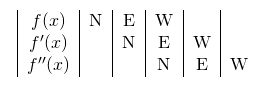
\includegraphics[width=0.4\textwidth]{images/grafisch_ableiten_tabelle.PNG}
  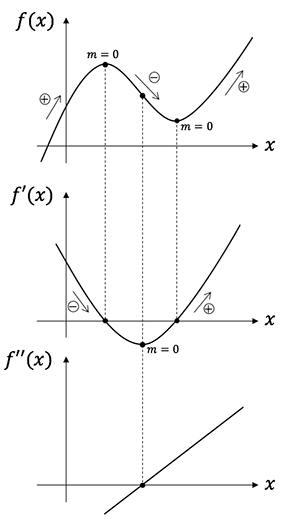
\includegraphics[width=0.3\textwidth]{images/grafisch_ableiten.PNG}
\end{figure}	

Die Nullstelle der 2. Ableitung $f''(x)$ zeigt uns den $x$-Wert für den Extrempunkt der 1.Ableitung $f'(x)$. Dieser wiederum zeigt uns, wo die Ausgangsfunktion $f(x)$ seinen Wendepunkt hat.


\subsubsection*{ABC-Formel}

Die Gleichung ist

\begin{align*}
	ax^2 + bx + c = 0
\end{align*}

ABC-Formel:

\begin{align*}
	x_{1,2} = \frac{-b \pm \sqrt{b^2 - 4ac}}{2a}
\end{align*}

\subsubsection*{Ableitungsregeln}

\begin{itemize}
	\item Ableiten einer Konstanten\\
	
	$f(x) = C \rightarrow f'(x) = 0$\\
	Beispiel: $f(x) = 5 \rightarrow f'(x) = 0$ oder $f(x) = -8 \rightarrow f'(x) = 0$	
	
	\item Ableiten von $x$\\
	
	$f(x) = x \rightarrow f'(x) = 1$\\
	Beispiel: $f(x) = x + 5 \rightarrow f'(x) = 1$ oder $f(x) = x - 8 \rightarrow f'(x) = 1$
	
	\item Potenzregel\\
	
	$f(x) = x^p \rightarrow f'(x) = px^{p-1}$\\
	Beispiel: $f(x) = x^3 \rightarrow f'(x) = 3x^2$ oder $f(x) = x^{-5} \rightarrow f'(x) = -5x^{-6}$
	
	\item Faktorregel / Skalarregel\\
	
	$f(x) = c \cdot g(x) \rightarrow f'(x) = c \cdot g'(x)$\\
	Beispiel: $f(x) = 2x^3 \rightarrow f'(x) = 6x^2$ oder $f(x) = -4x^{-4} \rightarrow f'(x) = 16x^{-5}$
	
	\item Summen-/Differenzregel\\
	
	$f(x) = f(x) \pm g(x) \rightarrow f'(x) = f'(x) \pm g'(x)$\\
	Beispiel: $f(x) = x^3 + 2x - 5 \rightarrow f'(x) = 3x^2 + 2$
	
	\item Kettenregel/Kompositionsregel\\
	
	$(u(v(x)))' = u'(v(x)) \cdot v'(x)$: Aussere Ableitung mal innerer Ableitung\\
	Beispiel: $f(x) = (x^3 + 5x)^3 \rightarrow f'(x) = 3 \cdot (x^3 + 5x)^2 \cdot (3x^2 + 5)$
	
	\item Produktregel\\
	
	$(u \cdot v)' = u' \cdot v + u \cdot v'$\\
	Beispiel: $f(x) = (2x^3 - 5) \cdot \sqrt{x} \rightarrow f'(x) = 6x^2 \cdot \sqrt{x} + (2x^3 - 5) \cdot \frac{1}{2 \sqrt{x}}$
	
	\item Quotientenregel\\
	$(\frac{u}{v})' = \frac{u' \cdot v - u \cdot v'}{v^2}$\\
	Beispiel: $f(x) = \frac{x^3 + 2}{x^5}$\\
	$f'(x) = \frac{3x^2 \cdot x^5 - (x^3 + 2) \cdot 5x^4}{(x^5)^2} = \frac{3x^7 - 5x^7 - 10x^4}{x^{10}} = \frac{-2x^7 - 10x^4}{x^{10}}$\\
	
	\textbf{Tipp:} Manchmal kann man einen Bruch umformen und benötigt gar nicht die QUotientenregel! Schreibt den Bruch einfach als Produkt und wendet die Produktregel an.
	\item Reziprokenregel/Kehrwertregel\\
	
	$\left[ \frac{1}{f(x)}\right]' = - \frac{f'(x)}{f(x)^2}$\\
	Beispiel: $f(x) = \frac{1}{x^2 + 1} \rightarrow f'(x) = - \frac{2x}{(x^2 + 1)^2}$\\
	Beispiel: $f(x) = \frac{1}{cos(x)} \rightarrow f'(x) = - \frac{(-sin(x))}{cos^2(x)}$
	\item Inversenregel/Umkehrregel\\
	
	Die Inversenregel besagt, dass eine umkehrbare (das heisst bijektive) reele Funktion $f$, die an der Stelle x differenzierbar ist und dort keine waagerechte Tangente besitzt, d.h. fuer die $f'(x) \neq 0$ gilt,\\
	auch ihre Umkehrfunktion $f^{-1}$ an der Stelle $y = f(x)$ differenzierbar ist mit Ableitung
	
	\begin{align*}
		(f^{-1})'(y) = \frac{1}{f'(f^{-1}(y))} = \frac{1}{f'(x)}
	\end{align*}
	
Beispiel: Die Umkehrfunktion der Exponentialfunktion $y = f(x) = e^x$ ist der natürliche Logarithmus.\\

\begin{align*}
	f^{-1} = ln(y)
\end{align*}

Wegen $f'(x) = e^x$ gilt also

\begin{align*}
	ln'(y) = \frac{1}{e^x} = \frac{1}{y}
\end{align*}

Eine weitere wichtige Anwendung der Umkehrregel sind die Ableitungen der Umkehrfunktionen der trigonometrischen Funktionen. So gilt z.B. fuer die Ableitung der Arkussinus

\begin{align*}
	arcsin'(y) = \frac{1}{cos(arcsin(y))}
\end{align*}

Mit der Identitaet $cos^2(y) + sin^2(y) = 1$ folgt

\begin{align*}
	arcsin'(y) = \frac{1}{\sqrt{1 - sin^2(arcsin(y))}} = \frac{1}{\sqrt{1 - y^2}}
\end{align*}
	
	\item Ableiten von e-Funktionen\\
	
	Die offizielle Methode ist, dass man die Kettenregel anwendet. Die einfachere Methode funktioniert wie folgt:\\
	
	$(e^{\text{etwas}})' = e^\text{etwas} \cdot (etwas)'$\\
	
	Beispiel: $f(x) = e^{5x} \rightarrow f'(x) = e^{5x} \cdot 5$\\
	Beispiel: $f(x) = e^{2 - 4x} \rightarrow f'(x) = -4e^{2 - 4x}$ 
	
	\item Ableiten von ln-Funktionen\\
	
	Eine Voraussetzung um diese Methode anzuwenden ist, dass wir wissen, dass $f(x) = ln(x) \rightarrow f'(x) = \frac{1}{x}$\\
	
	$(ln(etwas))' = \frac{1}{etwas} \cdot (etwas)'$\\
	
	Beispiel: $f(x) = ln(5x^2 - 3x) \rightarrow f'(x) = \frac{1}{5x^2 - 3x} \cdot (5x^2 - 3x)' = \frac{1}{5x^2 - 3x} \cdot (10x - 3)$
\end{itemize}



\subsubsection*{Wichtige Ableitungen}

\begin{itemize}
	\item $(a^x)' = a^x \cdot ln(a)$ with special case $(e^x)' = e^x$
	\item $(log_ax)' = \frac{1}{x \cdot ln(a)}$ with special case $(ln(x))' = \frac{1}{x}$
	\item $(sin(x))' = cos(x)$
	\item $(cos(x))' = -sin(x)$
	\item $(-sin(x))' = -cos(x)$
	\item $(-cos(x))' = sin(x)$
	\item $(tan(x))' = (\frac{sin(x)}{cos(x)})' = \frac{1}{cos^2(x)}$
	\item $(arcsin(x))' = \frac{1}{\sqrt{x - x^2}}$ where $arcsin = sin^{-1}$
	\item $(arccos(x))' = \frac{-1}{\sqrt{1 - x^2}}$ where $arccos = cos^{-1}$
	\item $(arctan(x))' = \frac{1}{1 + x^2}$ where $arctan = tan^{-1}$
\end{itemize}


\subsubsection*{Trigonometrische Identitaeten}

\begin{itemize}
	\item $sin^2(x) + cos^2(x) = 1$
	\item $sin(2x) = 2 sin(x)cos(x)$
	\item $cos(2x) = cos^2(x) - sin^2(x)$
\end{itemize}

Summenregeln

\begin{itemize}
	\item $sin(x + y) = sin(x)cos(y) + cos(x)sin(y)$
	\item $cos(x + y) = cos(x)cos(y) - sin(x)sin(y)$
	\item $sin(x - y) = sin(x)cos(y) - cos(x)sin(y)$
	\item $cos(x - y) = cos(x)cos(y) + sin(x)sin(y)$
\end{itemize}



\subsection*{Analysis - Integrale}



\subsubsection*{Wichtige Integrale}

\begin{itemize}
	\item $\int 0 \; dx = C$
	\item $\int a \; dx = ax + C$ so $\int 1 \; dx = x + C$
	\item $\int x^n \; dx = \frac{1}{n + 1} \cdot x^{n + 1} + C$, for $n \neq -1$
	\item $\int \frac{1}{x} \; dx = ln(x) + C$
	\item $\int e^x \; dx = e^x + C$
	\item $\int a^x \; dx = e^x + C$
	\item $\int a^x \; dx = \frac{1}{ln(a)} \cdot a^x + C$
	\item $\int sin(x) \; dx = - cos(x) + C$
	\item $\int cos(x) \; dx = sin(x) + C$
	\item $\int $
\end{itemize}


\end{document}
